\documentclass[a4paper,10pt]{report}
\usepackage[utf8]{inputenc}
\usepackage[T1]{fontenc}
\usepackage{graphicx}
\usepackage[francais]{babel}
\usepackage{hyperref}
\usepackage{color}
\usepackage{algpseudocode}
\usepackage{algorithm}
\usepackage{mathtools}


% Title Page
\title{Relations de voisinage et stratégies d'exploration}
\author{Adrien DROGUET}
\date{Avril - Juin 2014}

\pagestyle{plain}

\begin{document}
\maketitle
%customiser page de titre
%ajouter nom de l'encadrant
%logo univ

\tableofcontents
\pagebreak

\chapter*{Introduction}
\section*{Définitions}
\begin{itemize}
 \item \textbf{Problème :} Ensemble de villes devant être parcourues.
 \item \textbf{Voisinage :} Chemin parcourant toutes les villes sans répétition.
Solution au problème du voyageur de commerce.
 \item \textbf{Voisin améliorant :} Chemin voisin d'une solution X, dont le coût
est inférieur au coût de X.
 \item \textbf{Recherche locale :} Exploration exhaustive de l'ensemble des
voisins d'une solution donnée.
 Coûteux en temps d'exécution.
 \item \textbf{Relation de voisinage :} Fonction permettant de passer d'un
voisinage à un autre.
 \begin{itemize}
  \item \textit{\textbf{Swap :}} Échange la position de deux villes dans un
chemin.
  \item \textit{\textbf{Insert :}} Insert une ville avant une autre.
  \item \textit{\textbf{Reverse :}} Inverse un sous section d'un chemin.
 \end{itemize}
 \item \textbf{Stratégie de sélection :} Détermine la manière dont on choisit un
voisin en recherche locale.
 \begin{itemize}
  \item \textit{\textbf{First Fit :}} Choisir le premier voisin améliorant
trouvé.
  \item \textit{\textbf{Best Fit :}} Choisir le meilleur améliorant trouvé.
  \item \textit{\textbf{Worst Fit :}} Choisir le moins bon améliorant trouvé.
 \end{itemize}
\end{itemize}


\pagebreak
\section*{Introduction}

\paragraph{}
  Le voyageur de commerce est un problème bien connu dans le milieu informatique
: pour un ensemble de villes, minimiser la distance requise qu'un individu doit
parcourir afin de visiter chaque ville. De nombreuses études ont été menées sur
ce sujet et une quantité significative d'algorithmes de résolution ont été
définis au fil des ans. Pour cette raison, cette problématique forme un cadre
intéressant pour l'analyse de l'efficacité des différentes relations que l'ont
cherche à étudier.

\paragraph{} % sujet
  Le but de ce projet est d'étudier l'efficacité de différentes recherches de
voisinage et stratégies applicables à la résolution de ce problème en recherche
locale. Suite à l'étude des résultats de ces différents algorithmes et
stratégies, le projet vise la mise en place de méthodes permettant d'effectuer
une recherche partielle capable d'obtenir des résultats comparables à ceux d'une
recherche locale à un coût moindre en temps de calcul.


\paragraph{} % ressources utilisées
  Pour référence, nous avons utilisé les problèmes fourni par
\href{https://www.iwr.uni-heidelberg.de/groups/comopt/software/TSPLIB95/}{TSPLIB
}
- une bibliothèque d'échantillons d'instances pour le TSP (et autres problèmes
liés) provenant de diverses sources et de types variés. Dans notre cas, nous
nous sommes confiné à des problèmes symétriques à deux dimensions, avec des
distances entières ou réelles.


%%%%%%%%%%%%%%%%%%%%
% Partie Recherche %
%%%%%%%%%%%%%%%%%%%%
\part{Recherche}
\chapter{Recherche locale}

\paragraph{}
  Le \textit{Traveling Salesman Problem} est un problème d'optimisation
combinatoire : Soit un chemin $C$ de $n$ villes, avec $x_k, k \in [1, n]$ une
ville quelconque et $c_l, l \in [1, n]$ le numéro de la ville située à l'indice
$l$ du chemin $C$ tel que $c_l \in [1,n]$, et $d(x_i,x_j), i,j \in [1,n]$ la
distance entre la ville $i$ et la ville $j$.
\paragraph{}
  On cherche à minimiser {\Large $\sum_{i=1}^{n - 1} d(x_{c_i},x_{c_{i+1}})$}
en appliquant un algorithme de recherche locale.

\begin{algorithm}
  \begin{algorithmic}
    \Require $solution$ : Solution courante
    \Require $solutions$ : ensemble des solutions retenues
    \Require $voisins$ : ensemble des solutions voisines de $solution$
    \Require $solutionAmeliorante(actuelle, nouvelle)$ : fonction d'évaluation
booléenne renvoyant vrai si une solution est considérée de meilleure qualité
    \Require $solutionOptimale(solutions)$ : fonction renvoyant la solution
jugée plus appropriée pour la suite de la recherche dans un ensemble de
solutions
    \State
    \State $solutions \gets \emptyset$
    \For {$voisin \in voisins$}
      \If {\Call{solutionAmeliorante}{solution, voisin}}
	\State $solutions \gets solutions \cup voisin$
      \EndIf
    \EndFor
    \State $solution \gets$ \Call{solutionOptimale}{solutions}
  \end{algorithmic}
  \caption{Algorithme de recherche locale}
\end{algorithm}

\paragraph{}
  Notre projet propose plusieurs manière d'obtenir un voisinage, ainsi que
diverses façons d'évaluer une solution comme étant optimale pour la suite de la
recherche.

\section{Implémentation des algorithmes}
\subsection{Relations de voisinage}

\subsubsection{Déplacement}
\paragraph{}
  Après avoir établi une représentation satisfaisante et un système de lecture
des données fonctionnel (voir section 3.1), nous avons défini trois types de
mouvements, ou relation de voisinage à appliquer à une solution : l'échange
(Swap), l'insertion (Insert) et l'inversion (Reverse). Soient $C_i$ et $C_j$ les
villes aux indices $i$ et $j$ du chemin $C$ respectivement. Appliquons nos
relations de voisinage sur $C_i$ et $C_j$ pour obtenir le chemin $C^{'}$ :

\paragraph{}
\begin{itemize}
  \item \textbf{Swap :} On échange la position de $C_i$ et $C_j$.
  \begin{figure}[H]
    \begin{center}
      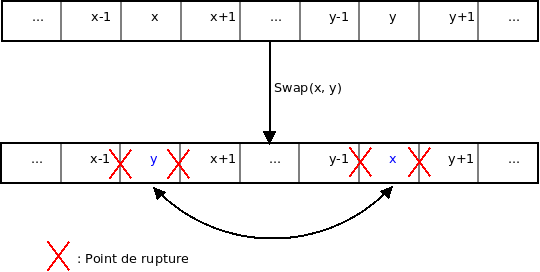
\includegraphics[width=\textwidth]{images/Swap.png}
    \end{center}
    \caption{Voisinage Swap}
  \end{figure}

  \item \textbf{Insert :} On insère $C_i$ avant $C_j$.
  \begin{figure}[H]
    \begin{center}
      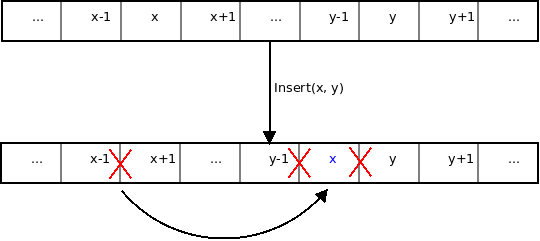
\includegraphics[width=\textwidth]{images/Insert.png}
    \end{center}
    \caption{Voisinage Insert}
  \end{figure}

  \item \textbf{Reverse :} On inverse la position de chaque ville entre $C_i$ et
$C_j$. $C^{'}_i \gets C_j$, $C^{'}_{i+1} \gets C_{j-1}$, ..., $C^{'}_{j-1} \gets
C_{i+1}$, $C^{'}_j \gets C_i$.
  \begin{figure}[H]
    \begin{center}
      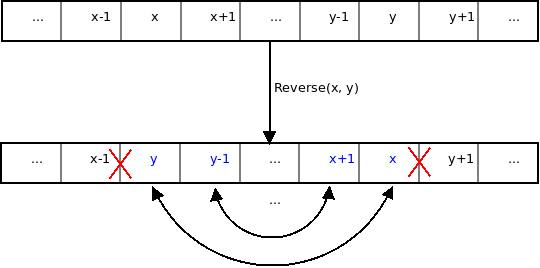
\includegraphics[width=\textwidth]{images/Reverse.png}
    \end{center}
    \caption{Voisinage Reverse}
  \end{figure}

\end{itemize}

\subsubsection{Variation de coût}
\paragraph{}
  Vous noterez les croix rouges séparant certaines villes sur les schémas
précédents. Ces celles-ci représentent ce que l'on appelle des points de
rupture, c'est à dire des changements dans la distance à parcourir, donc un
changement du coût de la solution (coût = distance que le voyageur doit
parcourir pour un chemin donné).
\paragraph{}
Afin d'éviter de recalculer le coût d'une solution, à chacune de ces relations
est associé une fonction de calcul de coût potentielle. Celle-ci prend en
paramètre les villes sur lesquels seront appliqués les déplacements, et effectue
les calculs aux points de rupture du chemin modifié.


\subsection{Stratégies de sélection d'un voisinage}

\paragraph{}
  Une fois que l'on dispose d'une fonction permettant de calculer le voisinage
d'une solution donnée, il faut déterminer une stratégie d'amélioration à
appliquer. Nous avons retenu trois stratégies distinctes à appliquer à notre
recherche locale : choisir le premier voisin améliorant que l'on trouve (First
Fit), choisir le meilleur voisin améliorant après avoir parcouru l'ensemble des
voisins possibles (Best Fit), ou bien choisir le voisin améliorant le moins
possible la solution actuelle (Worst Fit).

% algos d'exemples


\subsection{Lancement}

\paragraph{}
  Suite au parsage d'un TSP particulier, notre algorithme s'efforce d'appliquer
chacune des relations et chacune des stratégies spécifiées l'une après l'autre,
en partant éventuellement du même point de départ. Chaque voisinage est généré
aléatoirement à partir des données du problème, bien que dans le cas des
stratégies \textit{Best Fit} et \textit{Worst Fit}, on va chercher à explorer
l'ensemble des voisins possibles.

\paragraph{}
En fin d'exécution, un résumé des résultats obtenus est affiché en console.

\begin{figure}[h]
Run Results for a280:
 \begin{center}
Run Data: Relation=Reverse;	Strategy=First Fit;	starting cost=34194,
  end cost=3026;	depth=1182;	run time= 0.448 sec\linebreak
Run Data: Relation=Reverse;	Strategy=Best Fit;	starting cost=34194,
  end cost=2935;	depth=297;	run time= 9.652 sec\linebreak
Run Data: Relation=Reverse;	Strategy=Worst Fit;	starting cost=34194,
  end cost=3010;	depth=29699;	run time= 22 min 32.312 sec\linebreak
 \end{center}
  \label{a280-sample-results}
  \caption{Résumé de fin d'exécution - format texte}
\end{figure}

\paragraph{}
Instances utilisées (par ordre de lancement) :
\begin{itemize}
  \item \textbf{a280.tsp} : Instance principalement utilisée par les tests
unitaires, d'une taille respectable, mais pas excessive.
  \item \textbf{att48.tsp} : Instance de petite taille, utilisée lors de tests
manuels rapide ou en débuggage.
  \item \textbf{berlin52.tsp} : Instance de petite taille.
  \item \textbf{ali535.tsp} : Instance de grande taille, beaucoup utilisée
étalon lorsque l'on cherche à améliorer les temps d'exécution.
  \item \textbf{ch130.tsp} : Instance de taille moyenne.
  \item \textbf{ch150.tsp} : Instance de taille moyenne.
  \item \textbf{burma14.tsp} : Instance de très petite taille.
  \item \textbf{bier127.tsp} : Instance de taille moyenne, parfois substituée à
a280 dans les tests.
  \item \textbf{brd14051.tsp} : Instance de taille excessive, seule la stratégie
\textit{First Fit} met un temps "raisonnable" à atteindre un optimum local.
\textit{Best Fit} et \textit{Worst Fit} n'ont jamais été testé sur cette
instance.
\end{itemize}

\pagebreak
\section{Analyse et comparaison de l'efficacité des algorithmes}
\subsection{Enregistrement des résultats}

\paragraph{}
  Après chaque exécution, on en enregistre les résultats dans des fichiers sous
forme textuelle. On distingue deux types de fichiers de sortie. D'une part les
*.results sont équivalents à la sortie console en fin d'exécution et
fournissent un résumé facile à lire pour les humains.
\paragraph{}
  D'autre part, les *.csv contiennent les mêmes données enregistrées au format
Comma Separated Value, ie. valeurs séparées par virgule, chaque ligne
correspondant à un couple Relation/Stratégie. Typiquement, le contenu de ces 
fichiers est concatené dans un fichier résumé, qui peut alors être copié tel
quel dans un tableur type Microsoft Excel ou Libre Office Calc. Voir en annexe
pour une description plus approfondie du tableur utilisé.

\begin{figure}[h]
  \begin{center}
    \begin{tabular}{cccrrrr}
      a280, &Reverse, &First Fit, &34194, &3026, &1182, &0.448\\
      a280, &Reverse, &Best Fit,  &34194, &2935, &297,  &9.652\\
      a280, &Reverse, &Worst Fit, &34194, &3010, &29699,&1352.312\\
    \end{tabular}
  \end{center}
  \label{a280-sample-csv}
  \caption{Résumé de fin d'exécution - format .csv}
\end{figure}

\subsection{Efficacité constatée}

\begin{figure}[h]
  \begin{center}
    \begin{tabular}{ccrrr}
      \textbf{Relation}& \textbf{Stratégie}& \textbf{Coût}& \textbf{Tps
d'exécution}& \textbf{Profondeur}\\
%     Relation&	Stratégie&	Coût Moyen&	Temps d'exécution&
%Profondeur\\
      Swap&	First Fit&	35 404,39&	107,186&	150 717\\
      Swap&	Best Fit&	37 313,41&	1 198,021&	46 680\\
      Swap&	Worst Fit&	33 743,71&	63 440,385&	3 275 847\\
      Insert&	First Fit&	28 531,77&	55,669&		144 553\\
      Insert&	Best Fit&	29 643,06&	233,594&	22 209\\
      Insert&	Worst Fit&	28 420,68&	65 041,299&	4 667 846\\
      Reverse&	First Fit&	25 823,20&	88,784&		148 971\\
      Reverse&	Best Fit&	25 344,58&	409,759&	16 198\\
      Reverse&	Worst Fit&	26 349,78&	58 323,618&	3 912 314\\
    \end{tabular}
  \end{center}
  \label{recap-general}
  \caption{Exemple de données générales recueillies après 40 exécutions sur
chaque instance}
\end{figure}

% résultats spécifiques

\begin{figure}[h]
  \begin{center}
    \begin{tabular}{|l|r|r|r|}
      \hline
      &		\textbf{First Fit}&	\textbf{Best Fit}&	\textbf{Worst
Fit}\\\hline
      \textbf{Swap}&	
	  7 653,780&
	  8 516,976&
	  \textbf{\textcolor{blue}{6 437,415}}\\\hline
      \textbf{Insert}&
	  5 435,000&
	  5 674,415&
	  \textbf{\textcolor{blue}{4 969,829}}\\\hline
      \textbf{Reverse}&
	  4 508,780&
	  \textbf{\textcolor{blue}{4 346,805}}&
	  4 532,195\\\hline
    \end{tabular}
    \label{a280-results}
    \caption{Résultats moyens pour le TSP a280}
  \end{center}
\end{figure}

\begin{figure}[h]
  \begin{center}
    \begin{tabular}{|l|r|r|r|}
      \hline
      &		\textbf{First Fit}&	\textbf{Best Fit}&	\textbf{Worst
Fit}\\\hline
      \textbf{Swap}&
	  3 200,600&
	  3 432,550&
	  \textbf{\textcolor{blue}{2 662,600}}\\\hline
      \textbf{Insert}&
	  2 516,450&
	  3 299,950&
	  \textbf{\textcolor{blue}{2 359,950}}\\\hline
      \textbf{Reverse}&
	  \textbf{\textcolor{blue}{861,250}}&
	  861,350&
	  861,400\\\hline
    \end{tabular}
    \label{ali535-results}
    \caption{Résultats moyens pour le TSP ali535}
  \end{center}
\end{figure}

\begin{figure}[h]
  \begin{center}
    \begin{tabular}{|l|r|r|r|}
      \hline
      &		\textbf{First Fit}&	\textbf{Best Fit}&	\textbf{Worst
Fit}\\\hline
      \textbf{Swap}&
	  53 327,317&
	  55 026,098&
	  \textbf{\textcolor{blue}{51 228,220}}\\\hline
      \textbf{Insert}&
	  44 155,293&
	  44 656,390&
	  \textbf{\textcolor{blue}{43 567,049}}\\\hline
      \textbf{Reverse}&
	  40 788,024&
	  \textbf{\textcolor{blue}{40 212,732}}&
	  40 826,512\\\hline
    \end{tabular}
    \label{att48-results}
    \caption{Résultats moyens pour le TSP att48}
  \end{center}
\end{figure}

\begin{figure}[H]
  \begin{center}
    \begin{tabular}{|l|r|r|r|}
      \hline
      &		\textbf{First Fit}&	\textbf{Best Fit}&	\textbf{Worst
Fit}\\\hline
      \textbf{Swap}&
	  \textbf{\textcolor{blue}{24,683}}&
	  25,756&
	  26,098\\\hline
      \textbf{Insert}&
	  26,098&
	  \textbf{\textcolor{blue}{24,585}}&
	  24,732\\\hline
      \textbf{Reverse}&
	  \textbf{\textcolor{blue}{23,659}}&
	  23,707&
	  24,390\\\hline
    \end{tabular}
    \label{burma14-results}
    \caption{Résultats moyens pour le TSP burma14}
  \end{center}
\end{figure}

\paragraph{}
Note: les résultats des autres TSP sont disponibles en annexe.

\paragraph{}
  Comme on peut le constater, le voisinage \textbf{\textit{Reverse}} est
nettement plus efficace que \textbf{\textit{Swap}} et \textbf{\textit{Insert}}.
En terme de stratégie, \textbf{Worst Fit} est la plus efficace combinée avec les
voisinages \textbf{\textit{Swap}} et \textbf{\textit{Insert}}, tandis que
\textbf{Best Fit} est la stratégie de choix pour \textbf{\textit{Reverse}}.

\chapter{Analyse d'efficacité et espérance d'amélioration}

\paragraph{}%revoir problématique
  Suite à l'étude préliminaire de l'efficacité de chacunes des relations et
stratégies, nous souhaitions étudier plus en détail le comportement de ces
algorithmes en cours d'exécution. En ayant une image plus nette des choix
effectués à un instant $t$ et de leur efficacité, on espère parvenir à
identifier des moyens d'améliorer l'efficacité des algorithmes déjà implémentés,
et/ou d'en souligner les avantages et limitations.

\paragraph{}
Nous nous sommes concentrés sur la relation de voisinage le plus efficace sur
l'ensemble de nos résultats : \textbf{\textit{Reverse}}. La première étape est
l'enregistrement de l'exécution de l'algorithme pas à pas.



\section{Enregistrement de l'exécution}
\subsection{Intégration dans le code existant}

\paragraph{}
  Avant toute chose, nous avons conçu de nouvelles structures permettant de
représenter l'état de notre algorithme à un instant \textit{t}. Ensuite, nous
avons greffé ces classes au code existant sans en modifier le comportement.
Finalement, nous avons choisi d'enregistrer chaque étape, chaque "pas" ligne par
ligne dans un fichier texte. Une fois encore, nous utilisons le format .csv afin
de pouvoir aisément transférer ces données dans un tableur au besoin.

\paragraph{}
  Via le tableur, nous établissons des graphes retraçant l'historique de chaque
exécution. La contrepartie de cette méthode est la relative difficulté à
comparer de nombreux résultats cote à cote, le logiciel n'étant pas bien adapté
pour traiter de tels volumes de données.

\subsection{Données enregistrées}

\paragraph{}
  Dans un premier temps, nous classons les relations de type \textit{Reverse}
en fonction de leur portée, c'est à dire le nombre d'éléments (villes) affectés.
On détermine ainsi de manière dynamique une série d'intervalles de taille
croissante pour chacune de nos instances. Nous avons mis en place deux manières
de créer nos intervalles : soit ils sont disjoints (voir tableau ci-dessous),
avec la borne inférieure égale à la borne supérieure de l'intervalle précédent ;
soit nous leur attribuons à tous la borne inférieure 1 (type retenu pour la
collecte des résultats). Le type et le taux de croissance peuvent être spécifiés
au lancement de l'application.

\begin{figure}[h]
  \begin{center}
    \begin{tabular}{cccccc}
      Reverse,&First Fit,&[1;4[,&[4;16[,&[16;64[,&[64;281[,\\
      Reverse,&First Fit,&0,    &0,     &1,      &1,\\
      Reverse,&First Fit,&0,    &0,     &2,      &1,\\
      Reverse,&First Fit,&0,    &0,     &2,      &2,\\
      Reverse,&First Fit,&0,    &0,     &2,      &3,\\
      Reverse,&First Fit,&0,    &0,     &2,      &4,\\
      Reverse,&First Fit,&0,    &0,     &2,      &5,\\
      Reverse,&First Fit,&0,    &0,     &3,      &5,\\
      Reverse,&First Fit,&0,    &0,     &3,      &6,\\
      Reverse,&First Fit,&0,    &0,     &3,      &7,\\
      Reverse,&First Fit,&0,    &0,     &3,      &8,\\
    \end{tabular}
  \end{center}
  \label{a280-sample-interval-simple}
  \caption{Extrait simplifié d'historique d'exécution - statistiques générales}
\end{figure}

\paragraph{}
  Dans un second temps, nous enregistrons les informations ayant trait à
l'exploration du voisinage et à l'action choisie. Ainsi, nous prenons note de
la portée de l'opération, de son degré d'amélioration (de combien le coût a
diminué), avec la quantité de voisins améliorants et de voisins dégradants
trouvés, accompagné du ratio voisins améliorants/voisins explorés.

\begin{figure}[h]
  \begin{tabular}{lcccl}
    Range,		&Cost diff,	
				&Stats,	&improv/degrad actions	&ratio,\\
    (23  ; 143),120,	&104,	&Stats:,	&1,2,		&0.333333,\\
    (117 ; 26),  59,	&788,	&Stats:,	&1,4,		&0.2,\\
    (117 ; 14),  47,	&106,	&Stats:,	&1,2,		&0.333333,\\
    (137 ; 81),  94,	&322,	&Stats:,	&1,1,		&0.5,\\
    (132 ; 22),  40,	&466,	&Stats:,	&1,7,		&0.125,\\
    (137 ; 81),  94,	&600,	&Stats:,	&1,1,		&0.5,\\
    (82  ; 86),   4,	&108,	&Stats:,	&1,6,		&0.142857,\\
    (1   ; 14),  13,	&22,	&Stats:,	&1,8,		&0.111111,\\
    (25  ; 129),104,	&548,	&Stats:,	&1,10,		&0.0909091,\\
    (91  ; 80), 139,	&662,	&Stats:,	&1,0,		&0,\\
    (137 ; 81),  94,	&94,	&Stats:,	&1,1,		&0.5,\\
    (100 ; 50), 100,	&334,	&Stats:,	&1,8,		&0.111111,\\
  \end{tabular}
  \label{a280-sample-interval-simple-bis}
  \caption{Extrait simplifié d'historique d'exécution - détails actions}
\end{figure}


\pagebreak
\section{Analyse des résultats}

\begin{center}
  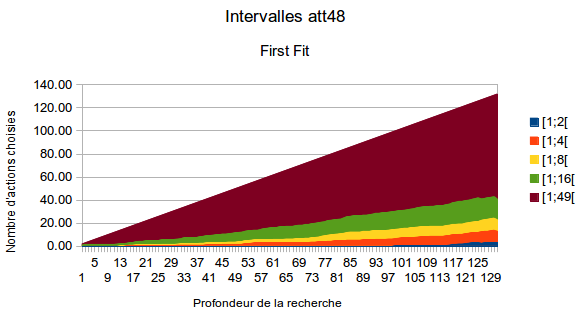
\includegraphics[width=\textwidth]{images/att48-intervals-first-fit.png}
\end{center}

\begin{center}
  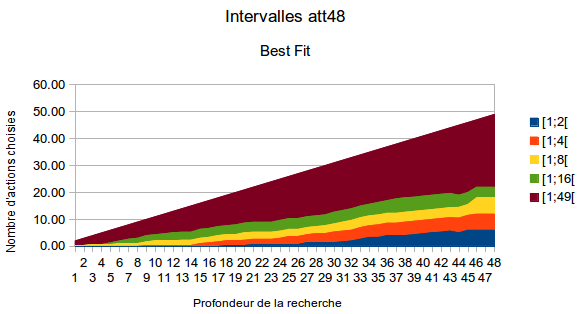
\includegraphics[width=\textwidth]{images/att48-intervals-best-fit.png}
\end{center}

\begin{center}
  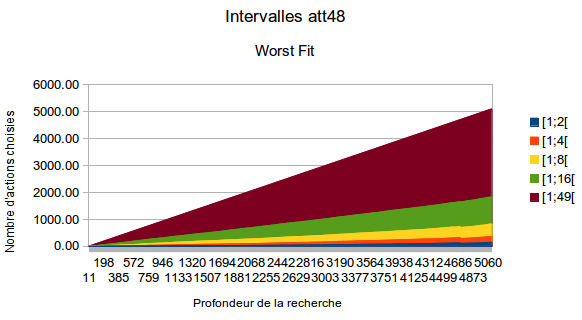
\includegraphics[width=\textwidth]{images/att48-intervals-worst-fit.png}
\end{center}

%insert graphs

%TODO: graphes intervalles pour ali535 \& bier127 (reste ds annexe) + graphes
%stats + commentaires

\section{Espérance d'amélioration - Implémentation d'un système de décision}

\paragraph{}
  Grâce aux résultats obtenus, il est possible d'analyser plus en profondeur le
comportement de nos voisinages et stratégies, et ainsi déterminer un système
permettant d'effectuer les recherches de manière plus intelligente. L'idée
directrice est d'avoir un ensemble de dispositifs permettant de jauger la
pertinence d'un voisinage donné en fonction des voisinages précédemment choisis.


\begin{figure}[h]
  \begin{tabular}{lll}
    Run Data: Relation=Reverse;&
      Strategy=First Fit;\\
      &starting cost=157894,&
      end cost=34817;\\
      &depth=135;\\
      &run time= 0.004 sec\\
    Run Data: Relation=Reverse;&
      Strategy=Best Fit;\\
      &starting cost=157894,&
      end cost=35155;\\
      &depth=46;\\
      &run time= 0.036 sec\\
    Run Data: Relation=Reverse;&
      Strategy=Worst Fit;\\
      &starting cost=157894,&
      end cost=36260;\\
      &depth=5374;\\
      &run time= 3.913 sec\\
  \end{tabular}
  \caption{Résultats témoins}
\end{figure}


\subsection{Piste 1 : Probabilité de considérer un voisin}
\subsubsection{Idée}

\paragraph{}
À chaque intervalle est associé une probabilité. À chaque voisin est associé un
intervalle. Nous sélectionnons désormais nos voisins avec l'algorithme suivant :

\begin{algorithm}[h]
  \begin{algorithmic}
    \Require $voisins$ : ensemble de Voisin
    \ForAll{$voisin \in voisins$}
      \State $roll\gets \Call{valeurAleatoire}{}$
      \If{$roll \leq voisin.intervalle.probabilite$}
	\State $selection \gets voisin$
	\State sortir
      \EndIf
    \EndFor
    \If{\Call{satisfaitStrategie}{selection}}
      \Return selection
    \EndIf
  \end{algorithmic}
  \caption{Sélection probabiliste}
\end{algorithm}

\paragraph{}
\underline{Note :} La variable \textit{selection} peut avoir été modifiée par la
fonction \textit{satisfaitStrategie}, en fonction de la stratégie utilisée.

\paragraph{}
  On espère ainsi qu'une fois arrivé en milieu ou fin de recherche, on ignorera
des mouvements que l'on estime avoir peu de chances d'améliorer la solution
actuelle. La probabilité d'un intervalle évolue en fonction du nombre de voisins
acceptants qu'il produit.


\begin{algorithm}[h]
  \begin{algorithmic}
    \Require $selection$ : Voisin
    \Require $increment > 0$
    \State 
    \Comment{Voir description du calcul de l'incrément ci-dessous}
    \State $probabilite \gets selection.intervalle.probabilite$
    \If{$ameliorant(selection)$}
      \State $selection.intervalle.probabilite \gets probabilite + increment$
    \Else
      \State $selection.intervalle.probabilite \gets probabilite - increment$
    \EndIf
    \State ...
    \Comment{Suite de la procédure dépend du type de stratégie choisie}
    \Ensure $selection.intervalle.probabilite \leq 1$
  \end{algorithmic}
  \caption{satisfaitStrategie (Générique)}
\end{algorithm}

\paragraph{}
\underline{Note :} On modifie la probabilité d'un seul intervalle à la fois.
Alternativement, on peut choisir de n'effectuer qu'une seule condition de
changement de la probabilité (décroître si voisin non-améliorant).


\begin{figure}[h]
 \begin{tabular}{lll}
  Run Data:Relation=Reverse;&
    Strategy=First Fit;\\
    &starting cost=162567,&
    end cost=43234;\\
    &depth=141;\\
    &run time= 0.008 sec\\
  Run Data:Relation=Reverse;&
    Strategy=Best Fit;\\
    &starting cost=162567,&
    end cost=41921;\\
    &depth=47;\\
    &run time= 0.064 sec\\
  Run Data:Relation=Reverse;&
    Strategy=Worst Fit;\\
    &starting cost=162567,&
    end cost=104442;\\
    &depth=162;\\
    &run time= 0.199 sec\\
 \end{tabular}
 \caption{Résultats avec sélection probabiliste}
\end{figure}


\subsubsection{Problèmes}

\paragraph{}
  Dans notre cas, l'obtention d'un jet aléatoire prend plus de temps processeur
que de calculer le coût d'un voisin potentiel. On aura également des difficultés
à faire en sorte que les probabilités entre les différents intervalles soient
significatives sans évoluer trop rapidement. Une évolution trop rapide peut nous
amener à refuser tous les voisins d'une solution à une profondeur relativement
faible, ce qui peut s'avérer particulièrement problématique dans le cas de
\textit{Worst Fit}.
\paragraph{}
  Pour remédier en partie à cela, la formule d'évolution de la probabilité prend
en compte la taille du problème à traiter et la différence de coût par rapport à
la solution précédente.


\subsection{Piste 2 : Trier les intervalles}
\subsubsection{Idée}

\paragraph{}
  Étant donné que, d'après nos résultats d'exécution, les grands intervalles ont
tendance à être beaucoup plus intéressants en début et milieu de recherche, nous
avons cherché à orienter le chemin de la recherche. En modifiant les
probabilités de départ de chaque intervalle en fonction de leur taille (plus
grands = probabilité plus importante), on espère limiter le nombre d'analyses
"inutiles" en début de recherche.


\begin{algorithm}
  \begin{algorithmic}
    \Require $intervalles$ : ensemble d'Intervalle
    \Require $probleme$ : Problème
    \State 
    \Comment Note: $PROBA\_MIN$ : constante déterminant la probabilité minimum
qu'un
intervalle peut avoir avant le début de la recherche (par défaut 0,3)
    \State
    \State $nbrIntervalles \gets intervalles.taille$
    \State $pas \gets (1 - PROBA\_MIN) / probleme.taille$
    \State $probabilite \gets 1.0$
    \ForAll{$intervalle \in intervalles$}
      \State $intervalle.probabilite \gets probabilite$
      \State $probabilite \gets pas * (intervalle.borneMax -
intervalle.borneMin)$
    \EndFor
  \end{algorithmic}
  \caption{Ajustement des probabilités de départ}
\end{algorithm}


\begin{figure}[h]
 \begin{tabular}{lll}
  Run Data: Relation=Reverse;&
    Strategy=First Fit;\\
    &starting cost=164833,&
    end cost=36000;\\
    &depth=133;\\
    &run time= 0.007 sec\\
  Run Data: Relation=Reverse;&
    Strategy=Best Fit;\\
    &starting cost=164833,&
    end cost=39929;\\
    &depth=42;\\
    &run time= 0.061 sec\\
  Run Data: Relation=Reverse;&
    Strategy=Worst Fit;\\
    &starting cost=164833,&
    end cost=99563;\\
    &depth=157;\\
    &run time= 0.211 sec\\
 \end{tabular}
 \caption{Résultats avec sélection probabiliste orientée}
\end{figure}

\subsubsection{Problèmes}

\paragraph{}
  Une fois encore, on se heurte au coût des jets aléatoires. La problématique
de l'évolution des coûts reste présente. On note une amélioration marginale des
coûts de \textit{First Fit} et \textit{Best Fit}.


\subsection{Piste 2.5 : Tri / évolution fonction de la stratégie}

Note : Non implémenté.

\subsubsection{Idée}

\paragraph{}
  Deux idées: D'une part inverser la répartition des probabilités initiales
lorsque l'on a affaire à une stratégie \textit{Worst Fit}. D'autre part,
utiliser une formule d'évolution de la probabilité plus "douce" lorsque l'on
est en \textit{Worst Fit}, ou rendre la formule actuelle plus sensible à la
taille d'un pas.
  
\subsubsection{Problèmes potentiels}

\paragraph{}
  L'inversion des probabilités de départ peut n'avoir aucune incidence sur
la performance de \textit{Worst Fit}. Utiliser une formule générique pour chaque
stratégie semble préférable, mais trouver un bon équilibre entre tous les
paramètres de la formule (taux d'amélioration, portée de la modification) peut
s'avérer délicat.


\subsection{Piste 3 : Échantillonnage acceptable}

Note: Non implémenté.

\subsubsection{Idée}
  Au lieu d'explorer de manière exhaustive notre voisinage à chaque fois, on
ajoute un test du taux d'exploration en condition d'arrêt et de passage au
niveau suivant. On juge alors l'échantillon de voisin explorés jusqu'à ce moment
comme étant acceptable et on choisit le prochain point de départ pour le niveau
suivant de la recherche.

\paragraph{}
  Vraisemblablement, on devrait pouvoir définir le taux d'exploration au moment
de l'exécution de l'application. Il s'agirait alors d'optimiser le rapport taux
d'exploration / taille de l'instance de manière à obtenir des résultats
suffisamment proches de ceux de l'exploration exhaustive.

\paragraph{}
  En outre, ce système devrait être compatible à la fois avec l'exploration
probabiliste et la recherche locale classique.

\begin{algorithm}[H]
  \begin{algorithmic}
    \Require $voisins$ : ensemble de voisin
    \Require $solution$ : solution courante
    \Require $relation$ : relation de voisinage
    \Require $strategie$ : stratégie d'exploration
    \Require $ACCEPTANCE$ : constante du taux d'échantillon jugé acceptable
    \State
    \While{\Call{aVoisinsAmeliorant}{$solution, relation$}}
      \State $compteur \gets 0$
      \ForAll {$voisin \in voisins$}
	\State \Call{appliquerStrategie}{$strategie, solution, voisin$}
	\If{$(compteur / voisins.taille) \geq ACCEPTANCE$}
	  \State sortir
	\Else
	  \State $acceptance \gets \Call{augmenterAcceptance}{acceptance}$
	\EndIf
      \EndFor
      \If{$solution \neq strategie.voisinOptimal$}
	\Comment{une nouvelle solution a été trouvée}
	\State $solution \gets strategie.voisinOptimal$
      \Else
	\State sortir
      \EndIf
    \EndWhile
  \end{algorithmic}
  \caption{Exploration avec taux d'échantillonnage}
\end{algorithm}


\subsubsection{Problèmes potentiels}
Trouver un bon taux d'échantillonnage pourrait s'avérer difficile. Le problème
pourrait être résolu en déterminant le taux optimal au lancement de
l'application. Le problème devient alors de trouver une méthode de calcul
efficace.


%%%%%%%%%%%%%%%%%%%%
% Partie technique %
%%%%%%%%%%%%%%%%%%%%
\part{Développement}
\chapter{Architecture de l'application}

\paragraph{}
  Afin d'obtenir un programme à la fois rapide et faisant usage des propriétés
de la programmation orientée objet, le projet a été écrit en C++11.

\section{Structures de base}
\subsection{Représentation des données}
%core + parsage
\paragraph{}
  Les .tsp fournis par LIBTSP suivent assez rigoureusement la même structure de
fichier, ce qui les rend faciles à lire. Les objets \textbf{Problem} et
\textbf{City} forment le cœur de nos données et nous servent à faire abstraction
de certaines caractéristiques des différents TSP, principalement de la
représentation des coordonnées (nombres entiers ou réels). Voir la section
\textit{core} en annexe pour plus de détails.

\subsection{Compartimentalisation des algorithmes}
%relation & stratégies
\paragraph{}
  Afin de séparer au mieux les différentes voisinages et stratégies tout en
évitant autant que possible les duplications de code, nous tirons avantage du
polymorphisme et de l'héritage pour généraliser le traitement de ces objets.
Voir les diagrammes de classe dans les sections \textit{relation} et
\textit{strategy} en annexe.


\section{Exécution}
\subsection{Lancement des algorithmes}
%main, parser & runner
\paragraph{}
  Le programme s'exécute en ligne de commande avec un certain nombre d'arguments
obligatoires, tels que le nom du fichier .tsp ou les relations de voisinage et
stratégies à utiliser, et des arguments optionnels activant ou désactivant
certains contrôles ou écritures de trace. Une fois tous les objets créés et
configurés, le main passe la main à la classe \textit{Runner} (voir annexe).

\subsection{Analyse Comportementale}
%interval stuff
\paragraph{}
  Nous utilisons 3 classes afin d'enregistrer chaque pas de l'exécution de notre
algorithme: \textit{Action}, \textit{Interval} et \textit{IntervalManager}.
\textit{Action} mémorise quel voisin a été choisi et avec quel gain (ou perte)
par rapport à la solution actuelle. \textit{Interval} permet de classer ces
actions et \textit{IntervalManager} sert de chef d'orchestre. Du fait des
informations mises en mémoire par ces classes, les entités dédiées à la
recherche partielle en font également usage pour déterminer la pertinence d'un
voisinage.

\subsection{Recherche partielle}
%choice & hook
\paragraph{}
  L'organisation des classes de prise de décision est légèrement plus chaotique.
La classe \textit{ChoiceMaker} correspond à la première tentative d'analyse de
pertinence. Elle implémente l'interface \textit{Hookable} afin de s'interfacer
avec les classes de type \textit{Relation} sans causer de conflits d'inclusion
multiples. \textit{ChoicePicker} a un rôle similaire, implémente la même
interface et, du point de vue de \textit{Relation}, opère de la même manière
que \textit{ChoiceMaker}.


\chapter{Déroulement du projet}
\section{Organisation}
\subsection{Contrôle d'avancement}

\subsubsection{Gestion de version}
\paragraph{}
  Afin de pouvoir garder un contrôle optimal sur les changements et évolutions
du projet, nous avons adopté un système de contrôle de version Git, avec un
dépôt distant hébergé sur Github. Nous employons une approche type "commits
courants, commits courts", de diviser nos changements au mieux - ce qui facilite
les réversions lorsque l'on en a besoin.

\paragraph{}
  Combiné à un journal de bord personnel, l'historique des commits permet
d'avoir une vision d'ensemble précise de l'évolution de l'application.

\subsubsection{Rapports hebdomadaires et réunions}
\paragraph{}
  Chaque semaine, un compte-rendu de l'avancement, des difficultés rencontrées,
résultats obtenus et des évolutions à venir est rédigé, accompagné de réunions
dès qu'une étape importante est atteinte - implémentation des relations et
stratégie, des traces d'exécution, de la prise de décision...


\subsection{Contrôle de non-régression}
%tests unitaires
\paragraph{}
  La quasi-totalité des méthodes, fonctionnalités et bugs sont contrôlés par
une batterie de tests unitaires, mettant parfois en évidence une régression ou
un comportement incorrect. Ainsi, à chaque révision majeure ou en fin de
journée, on lance l'ensemble des tests pour vérifier qu'aucune anomalie n'a fait
surface (y compris dans les tests eux-mêmes).

%retro compatibilité
\paragraph{}
  On s'efforce également de maintenir un certain degré de rétrocompatibilité
: la plupart des nouvelles méthodes ou algorithmes doivent être activés lors de
l'appel en ligne de commande. Heureusement, le script de lancement permet de
maintenir une bonne utilisabilité de l'application malgré l'inflation du nombre
de paramètres optionnels.

\subsection{Profiling et Optimisation}
%valgrind, callgrind & autre
\paragraph{}
  Dans le but d'améliorer la vitesse d'exécution, l'utilisation mémoire de
l'application, et corriger des problèmes potentiels, nous tirons avantage des
capacités de \textbf{valgrind}, \textbf{callgrind} ainsi qu'une poignée de
contrôles manuels pour obtenir une image précise du comportement de notre
algorithme. Ces informations nous permettent ensuite d'optimiser certaines
sections du code lorsque le besoin se fait sentir.

\paragraph{}
  Ce type opération a donné naissance à certaines structures allégées, comme des
voisins simplifiés, ne contenant que les informations essentielles aux classes
dont elles sont attributs. On s'efforce de libérer dès que possible les données
ayant dépassé leur période d'utilité, rendant le programme beaucoup plus robuste
et capable de tenir la charge sur de grandes instances.


\section{Difficultés techniques}

\paragraph{}
  S'agissant du premier projet écrit en C++ de taille significative que j'ai eu
l'occasion de réaliser, la première partie du projet a été marqué par une série
de bugs qu'une plus grande familiarité avec le langage aurait pu éviter. En
particulier, un bug sévère passé inaperçu pendant quelques semaines rendait les
résultats alors obtenus nuls, forçant à relancer de nombreuses exécutions après
correction.

\paragraph{}
  Ceci a eu des conséquences importantes sur le temps de développement, forçant
à revoir à la baisse les ambitions du projet. Les algorithmes génétiques, le
changement de voisinage en cours de recherche et quelques autres concepts ont dû
être enlevé du planning.


\chapter*{Conclusion}
\section*{} %conclusion / rétrospective


\section*{Informations complémentaires}
%bibliographie
%licence
%repo github


\end{document}          
